% Options for packages loaded elsewhere
\PassOptionsToPackage{unicode}{hyperref}
\PassOptionsToPackage{hyphens}{url}
%
\documentclass[
  ignorenonframetext,
]{beamer}
\usepackage{pgfpages}
\setbeamertemplate{caption}[numbered]
\setbeamertemplate{caption label separator}{: }
\setbeamercolor{caption name}{fg=normal text.fg}
\beamertemplatenavigationsymbolsempty
% Prevent slide breaks in the middle of a paragraph
\widowpenalties 1 10000
\raggedbottom
\setbeamertemplate{part page}{
  \centering
  \begin{beamercolorbox}[sep=16pt,center]{part title}
    \usebeamerfont{part title}\insertpart\par
  \end{beamercolorbox}
}
\setbeamertemplate{section page}{
  \centering
  \begin{beamercolorbox}[sep=12pt,center]{part title}
    \usebeamerfont{section title}\insertsection\par
  \end{beamercolorbox}
}
\setbeamertemplate{subsection page}{
  \centering
  \begin{beamercolorbox}[sep=8pt,center]{part title}
    \usebeamerfont{subsection title}\insertsubsection\par
  \end{beamercolorbox}
}
\AtBeginPart{
  \frame{\partpage}
}
\AtBeginSection{
  \ifbibliography
  \else
    \frame{\sectionpage}
  \fi
}
\AtBeginSubsection{
  \frame{\subsectionpage}
}

\usepackage{amsmath,amssymb}
\usepackage{iftex}
\ifPDFTeX
  \usepackage[T1]{fontenc}
  \usepackage[utf8]{inputenc}
  \usepackage{textcomp} % provide euro and other symbols
\else % if luatex or xetex
  \usepackage{unicode-math}
  \defaultfontfeatures{Scale=MatchLowercase}
  \defaultfontfeatures[\rmfamily]{Ligatures=TeX,Scale=1}
\fi
\usepackage{lmodern}
\ifPDFTeX\else  
    % xetex/luatex font selection
\fi
% Use upquote if available, for straight quotes in verbatim environments
\IfFileExists{upquote.sty}{\usepackage{upquote}}{}
\IfFileExists{microtype.sty}{% use microtype if available
  \usepackage[]{microtype}
  \UseMicrotypeSet[protrusion]{basicmath} % disable protrusion for tt fonts
}{}
\makeatletter
\@ifundefined{KOMAClassName}{% if non-KOMA class
  \IfFileExists{parskip.sty}{%
    \usepackage{parskip}
  }{% else
    \setlength{\parindent}{0pt}
    \setlength{\parskip}{6pt plus 2pt minus 1pt}}
}{% if KOMA class
  \KOMAoptions{parskip=half}}
\makeatother
\usepackage{xcolor}
\newif\ifbibliography
\usepackage{svg}
\setlength{\emergencystretch}{3em} % prevent overfull lines
\setcounter{secnumdepth}{-\maxdimen} % remove section numbering


\providecommand{\tightlist}{%
  \setlength{\itemsep}{0pt}\setlength{\parskip}{0pt}}\usepackage{longtable,booktabs,array}
\usepackage{calc} % for calculating minipage widths
\usepackage{caption}
% Make caption package work with longtable
\makeatletter
\def\fnum@table{\tablename~\thetable}
\makeatother
\usepackage{graphicx}
\makeatletter
\def\maxwidth{\ifdim\Gin@nat@width>\linewidth\linewidth\else\Gin@nat@width\fi}
\def\maxheight{\ifdim\Gin@nat@height>\textheight\textheight\else\Gin@nat@height\fi}
\makeatother
% Scale images if necessary, so that they will not overflow the page
% margins by default, and it is still possible to overwrite the defaults
% using explicit options in \includegraphics[width, height, ...]{}
\setkeys{Gin}{width=\maxwidth,height=\maxheight,keepaspectratio}
% Set default figure placement to htbp
\makeatletter
\def\fps@figure{htbp}
\makeatother
% definitions for citeproc citations
\NewDocumentCommand\citeproctext{}{}
\NewDocumentCommand\citeproc{mm}{%
  \begingroup\def\citeproctext{#2}\cite{#1}\endgroup}
\makeatletter
 % allow citations to break across lines
 \let\@cite@ofmt\@firstofone
 % avoid brackets around text for \cite:
 \def\@biblabel#1{}
 \def\@cite#1#2{{#1\if@tempswa , #2\fi}}
\makeatother
\newlength{\cslhangindent}
\setlength{\cslhangindent}{1.5em}
\newlength{\csllabelwidth}
\setlength{\csllabelwidth}{3em}
\newenvironment{CSLReferences}[2] % #1 hanging-indent, #2 entry-spacing
 {\begin{list}{}{%
  \setlength{\itemindent}{0pt}
  \setlength{\leftmargin}{0pt}
  \setlength{\parsep}{0pt}
  % turn on hanging indent if param 1 is 1
  \ifodd #1
   \setlength{\leftmargin}{\cslhangindent}
   \setlength{\itemindent}{-1\cslhangindent}
  \fi
  % set entry spacing
  \setlength{\itemsep}{#2\baselineskip}}}
 {\end{list}}
\usepackage{calc}
\newcommand{\CSLBlock}[1]{\hfill\break\parbox[t]{\linewidth}{\strut\ignorespaces#1\strut}}
\newcommand{\CSLLeftMargin}[1]{\parbox[t]{\csllabelwidth}{\strut#1\strut}}
\newcommand{\CSLRightInline}[1]{\parbox[t]{\linewidth - \csllabelwidth}{\strut#1\strut}}
\newcommand{\CSLIndent}[1]{\hspace{\cslhangindent}#1}

\makeatletter
\@ifpackageloaded{caption}{}{\usepackage{caption}}
\AtBeginDocument{%
\ifdefined\contentsname
  \renewcommand*\contentsname{Table of contents}
\else
  \newcommand\contentsname{Table of contents}
\fi
\ifdefined\listfigurename
  \renewcommand*\listfigurename{List of Figures}
\else
  \newcommand\listfigurename{List of Figures}
\fi
\ifdefined\listtablename
  \renewcommand*\listtablename{List of Tables}
\else
  \newcommand\listtablename{List of Tables}
\fi
\ifdefined\figurename
  \renewcommand*\figurename{Figure}
\else
  \newcommand\figurename{Figure}
\fi
\ifdefined\tablename
  \renewcommand*\tablename{Table}
\else
  \newcommand\tablename{Table}
\fi
}
\@ifpackageloaded{float}{}{\usepackage{float}}
\floatstyle{ruled}
\@ifundefined{c@chapter}{\newfloat{codelisting}{h}{lop}}{\newfloat{codelisting}{h}{lop}[chapter]}
\floatname{codelisting}{Listing}
\newcommand*\listoflistings{\listof{codelisting}{List of Listings}}
\usepackage{amsthm}
\theoremstyle{definition}
\newtheorem{definition}{Definition}[section]
\theoremstyle{remark}
\AtBeginDocument{\renewcommand*{\proofname}{Proof}}
\newtheorem*{remark}{Remark}
\newtheorem*{solution}{Solution}
\newtheorem{refremark}{Remark}[section]
\newtheorem{refsolution}{Solution}[section]
\makeatother
\makeatletter
\makeatother
\makeatletter
\@ifpackageloaded{caption}{}{\usepackage{caption}}
\@ifpackageloaded{subcaption}{}{\usepackage{subcaption}}
\makeatother
\ifLuaTeX
  \usepackage{selnolig}  % disable illegal ligatures
\fi
\usepackage{bookmark}

\IfFileExists{xurl.sty}{\usepackage{xurl}}{} % add URL line breaks if available
\urlstyle{same} % disable monospaced font for URLs
\hypersetup{
  pdftitle={ECCCos from the Black Box},
  pdfauthor={Patrick Altmeyer; Mojtaba Farmanbar; Arie van Deursen; Cynthia C. S. Liem},
  hidelinks,
  pdfcreator={LaTeX via pandoc}}

\title{ECCCos from the Black Box}
\subtitle{Faithful Model Explanations through Energy-Based Conformal
Counterfactuals}
\author{\textbf{Patrick Altmeyer} \and Mojtaba Farmanbar \and Arie van
Deursen \and Cynthia C. S. Liem}
\date{2024-01-04}
\institute{Delft University of Technology}

\begin{document}
\frame{\titlepage}

\begin{frame}{Open Questions}
\phantomsection\label{open-questions}
\begin{enumerate}[<+->]
\tightlist
\item
  What makes a counterfactual \textbf{plausible}?
\item
  Why do we need plausibility?
\item
  Is plausibility all we need?
\item
  What makes models more \textbf{explainable}?
\end{enumerate}
\end{frame}

\begin{frame}{Plausibility}
\phantomsection\label{plausibility}
There's no consensus on the exact definition of plausibility but we
think about it as follows:

\begin{definition}[Plausible
Counterfactuals]\protect\hypertarget{def-plausible}{}\label{def-plausible}

Let \(\mathcal{X}|\mathbf{y}^+= p(\mathbf{x}|\mathbf{y}^+)\) denote the
true conditional distribution of samples in the target class
\(\mathbf{y}^+\). Then for \(\mathbf{x}^{\prime}\) to be considered a
plausible counterfactual, we need:
\(\mathbf{x}^{\prime} \sim \mathcal{X}|\mathbf{y}^+\).

\end{definition}
\end{frame}

\begin{frame}{Counter Example}
\phantomsection\label{counter-example}
\begin{columns}[T]
\begin{column}{0.5\textwidth}
\begin{itemize}
\tightlist
\item
  The counterfactual in Figure~\ref{fig-implausible} is valid: it has
  crossed the decision boundary.
\item
  But is it consistent with the data in the target class (blue)?
\end{itemize}
\end{column}

\begin{column}{0.5\textwidth}
\begin{figure}

\centering{

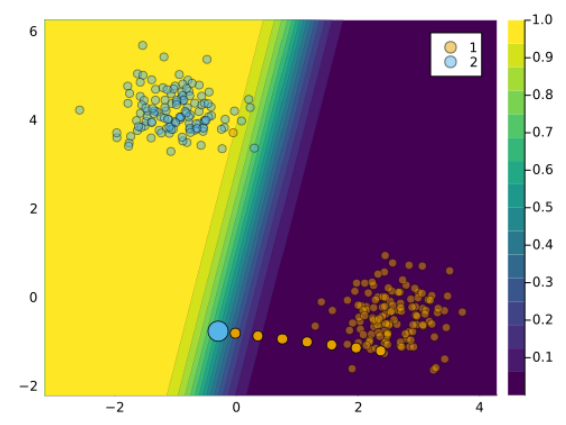
\includegraphics{www/implausible.png}

}

\caption{\label{fig-implausible}A valid but implausible counterfactual.
Source: Altmeyer, Deursen, and Liem (2023)}

\end{figure}%
\end{column}
\end{columns}
\end{frame}

\begin{frame}{Why Plausibility?}
\phantomsection\label{why-plausibility}
\begin{itemize}
\tightlist
\item
  Actionability: If a counterfactual is implausible, it is unlikely to
  be actionable.
\item
  Fairness: If a counterfactual is implausible, it is unlikely to be
  fair.
\item
  Robustness: If a counterfactual is implausible, it is unlikely to be
  robust.
\end{itemize}

\textbf{But}: Higher plausibility seems to require larger changes and
hence increase costs to individuals.
\end{frame}

\begin{frame}{Pick your Poison?}
\phantomsection\label{pick-your-poison}
All of these counterfactuals are valid explanations for the model's
prediction. Which one would you pick?

\begin{figure}

\centering{

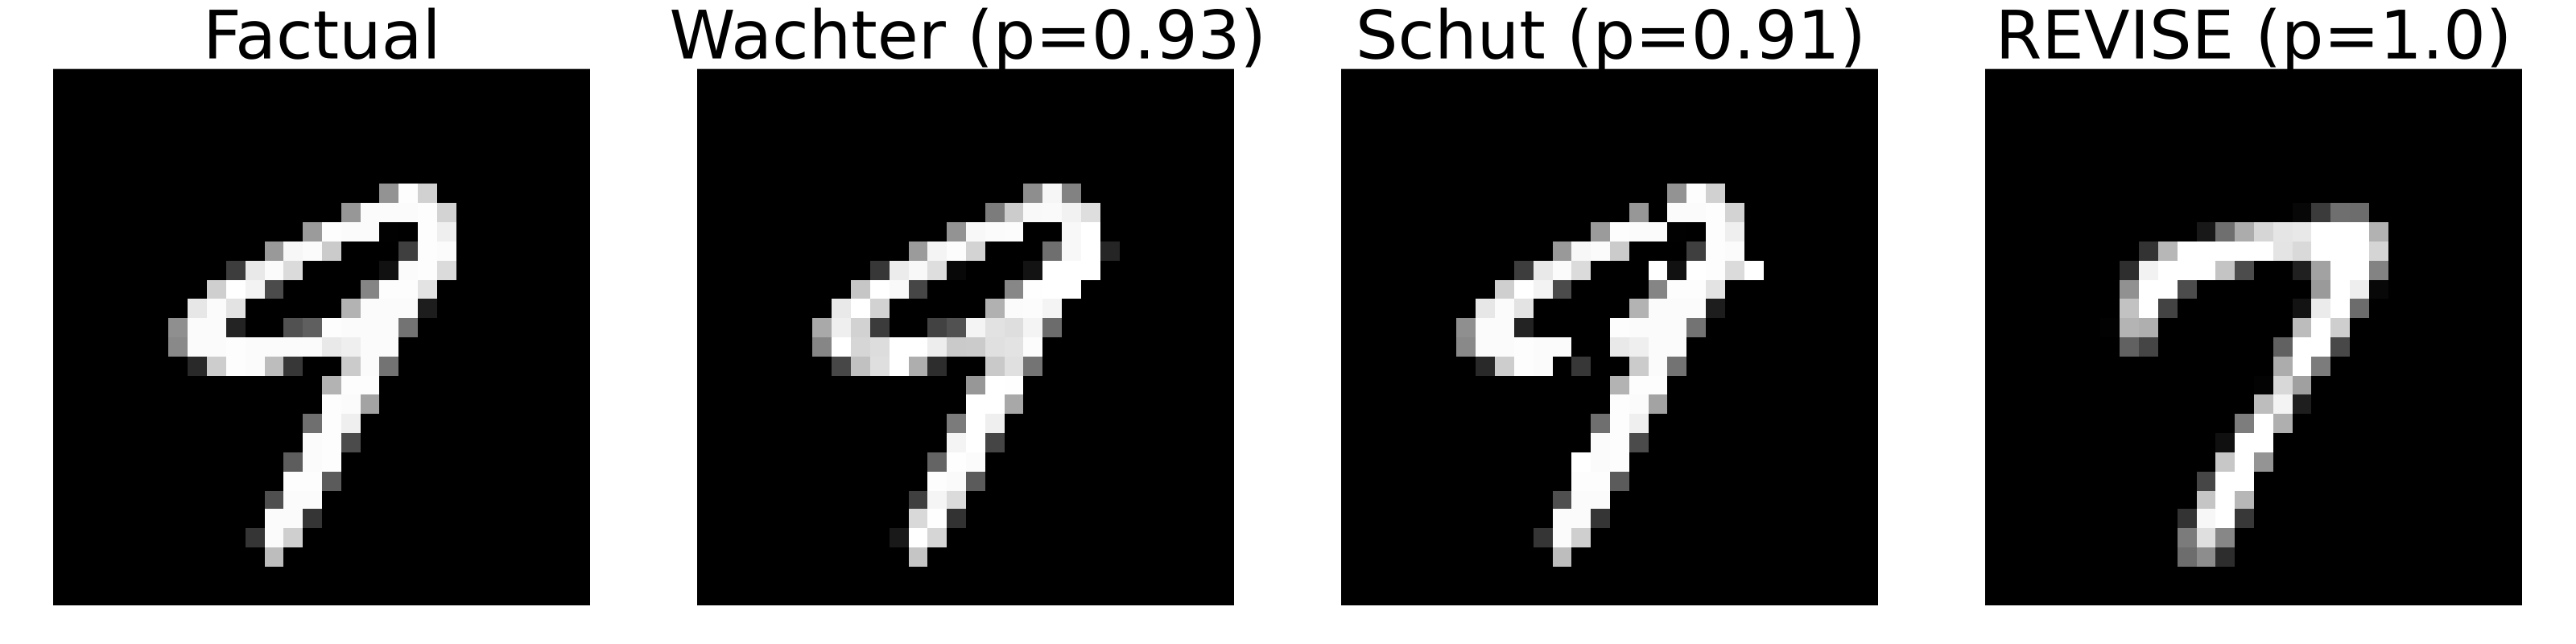
\includegraphics{www/poison.png}

}

\caption{\label{fig-cf-example}Turning a 9 into a 7: Counterfactual
Examplanations for an Image Classifier.}

\end{figure}%
\end{frame}

\begin{frame}{What do Models Learn?}
\phantomsection\label{what-do-models-learn}
These images are sampled from the posterior distribution learned by the
model. Looks different, no?

\begin{figure}

\centering{

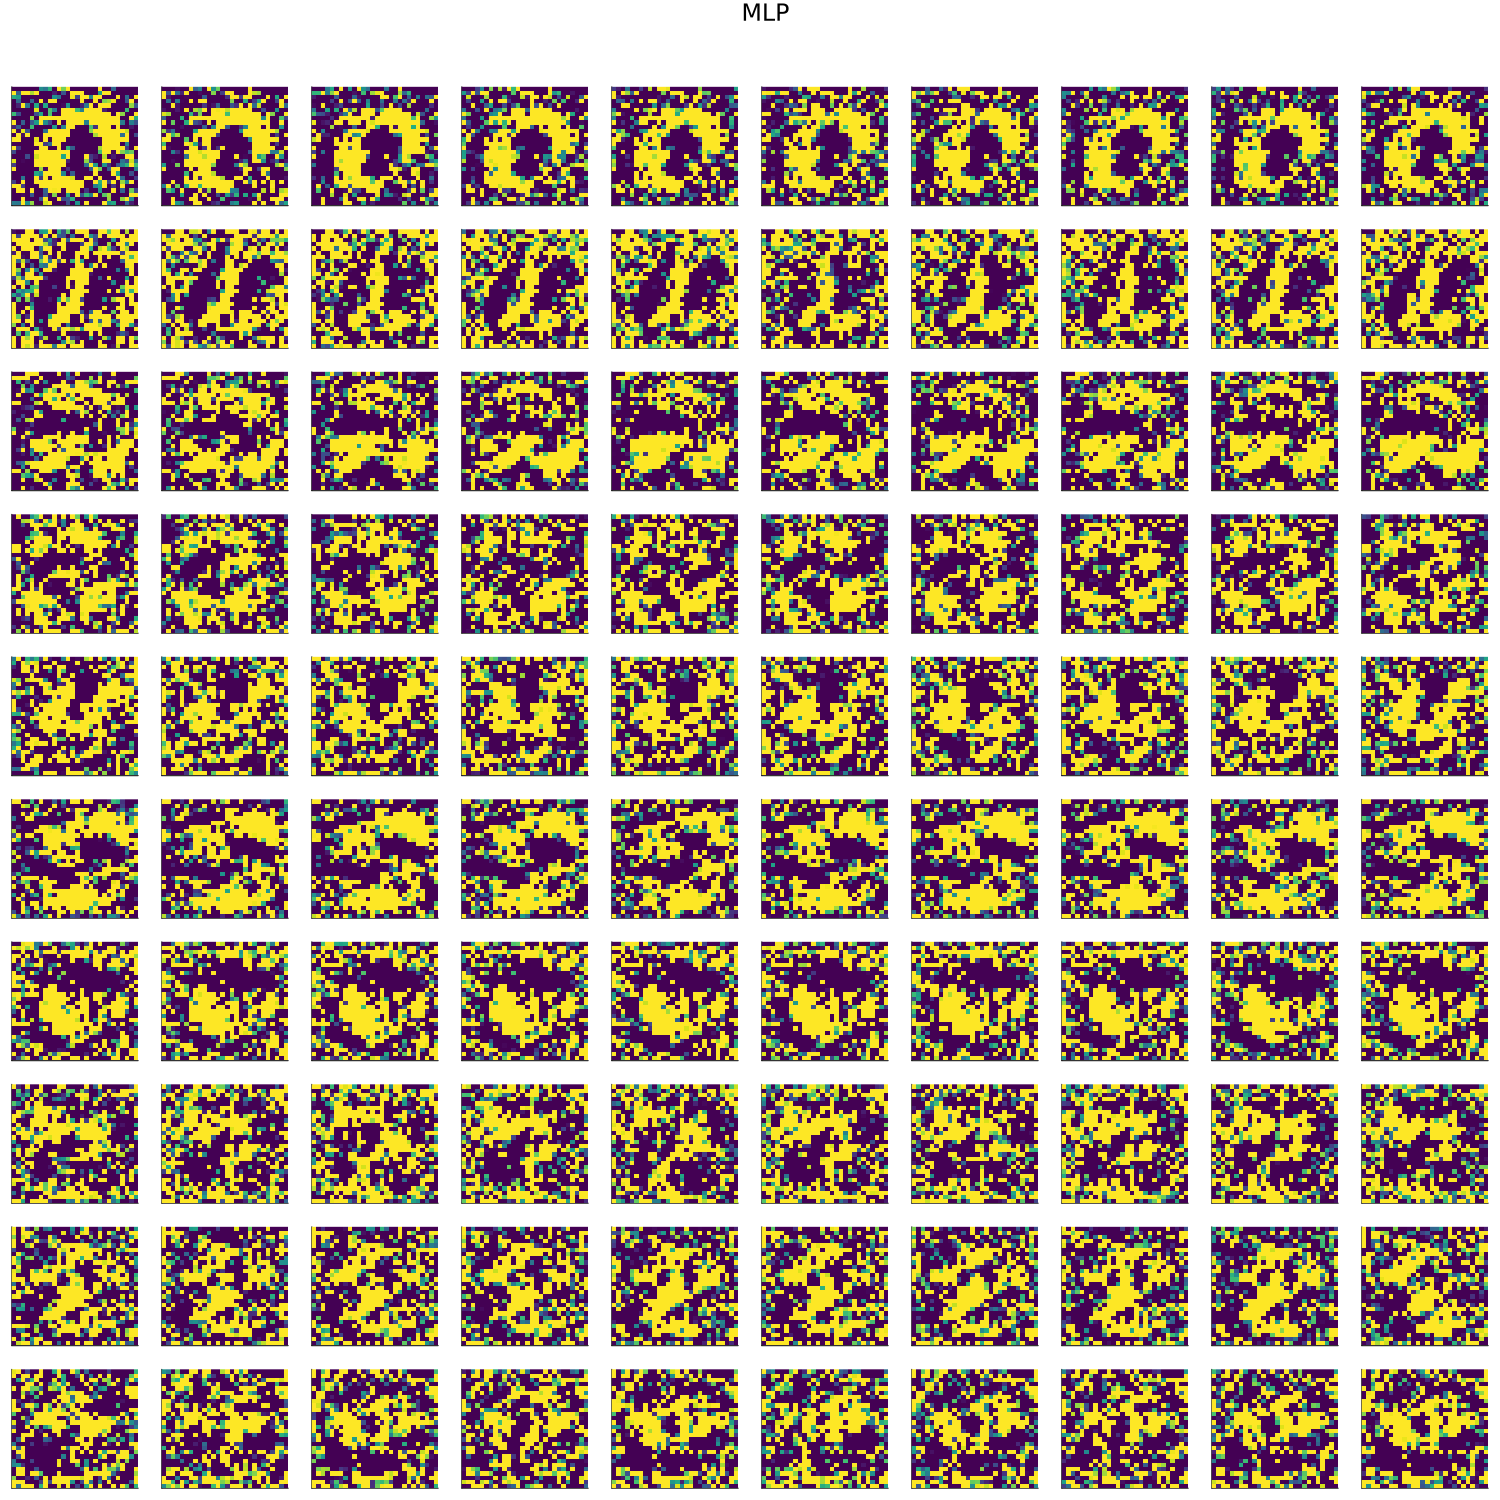
\includegraphics{www/learn.png}

}

\caption{\label{fig-learn}Conditional Generated Images from the Image
Classifier}

\end{figure}%
\end{frame}

\begin{frame}{Faithful Counterfactuals}
\phantomsection\label{faithful-counterfactuals}
\begin{columns}[T]
\begin{column}{0.6\textwidth}
We propose a way to generate counterfactuals that are as plausible as
the underlying model permits (under review).

\begin{definition}[Faithful
Counterfactuals]\protect\hypertarget{def-faithful}{}\label{def-faithful}

Let
\(\mathcal{X}_{\theta}|\mathbf{y}^+ = p_{\theta}(\mathbf{x}|\mathbf{y}^+)\)
denote the conditional distribution of \(\mathbf{x}\) in the target
class \(\mathbf{y}^+\), where \(\theta\) denotes the parameters of model
\(M_{\theta}\). Then for \(\mathbf{x}^{\prime}\) to be considered a
faithful counterfactual, we need:
\(\mathbf{x}^{\prime} \sim \mathcal{X}_{\theta}|\mathbf{y}^+\).

\end{definition}
\end{column}

\begin{column}{0.4\textwidth}
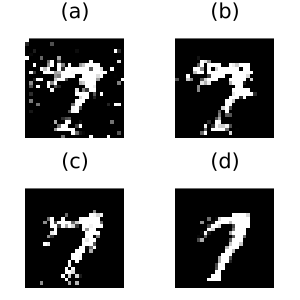
\includegraphics{www/mnist_eccco_new.png}
\end{column}
\end{columns}

\begin{figure}

\centering{

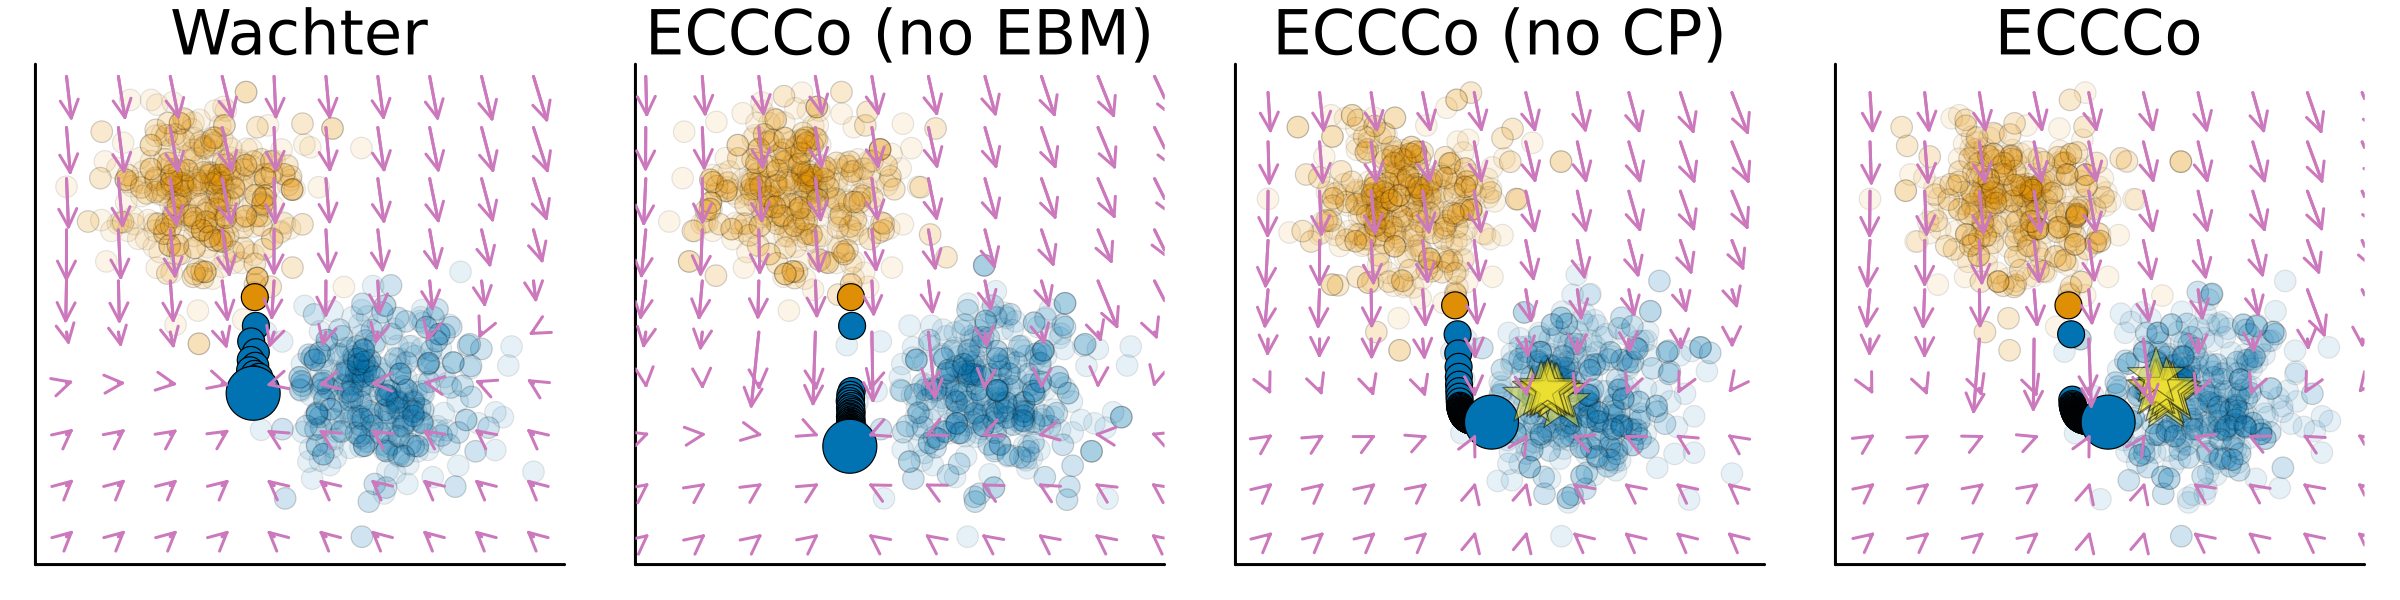
\includegraphics[width=0.65\textwidth,height=\textheight]{www/poc_gradient_fields.png}

}

\caption{\label{fig-poc-gradient-fields}Gradient fields and
counterfactual paths for different generators.}

\end{figure}%
\end{frame}

\begin{frame}{Improving Models}
\phantomsection\label{improving-models}
Now that we have a tool to faithfully explain models we may ask:
\textbf{how} do models learn plausible explanations? Initial evidence:

\begin{enumerate}
\tightlist
\item
  Incorporating predictive uncertainty (e.g.~ensembling).
\item
  Addressing robustness (e.g.~adversarial training in Schut et al.
  (2021)).
\item
  Better model architectures.
\item
  Hybrid modelling (i.e.~combining generative and discriminative
  models).
\end{enumerate}
\end{frame}

\begin{frame}{Example: Architecture}
\phantomsection\label{example-architecture}
\begin{figure}

\centering{

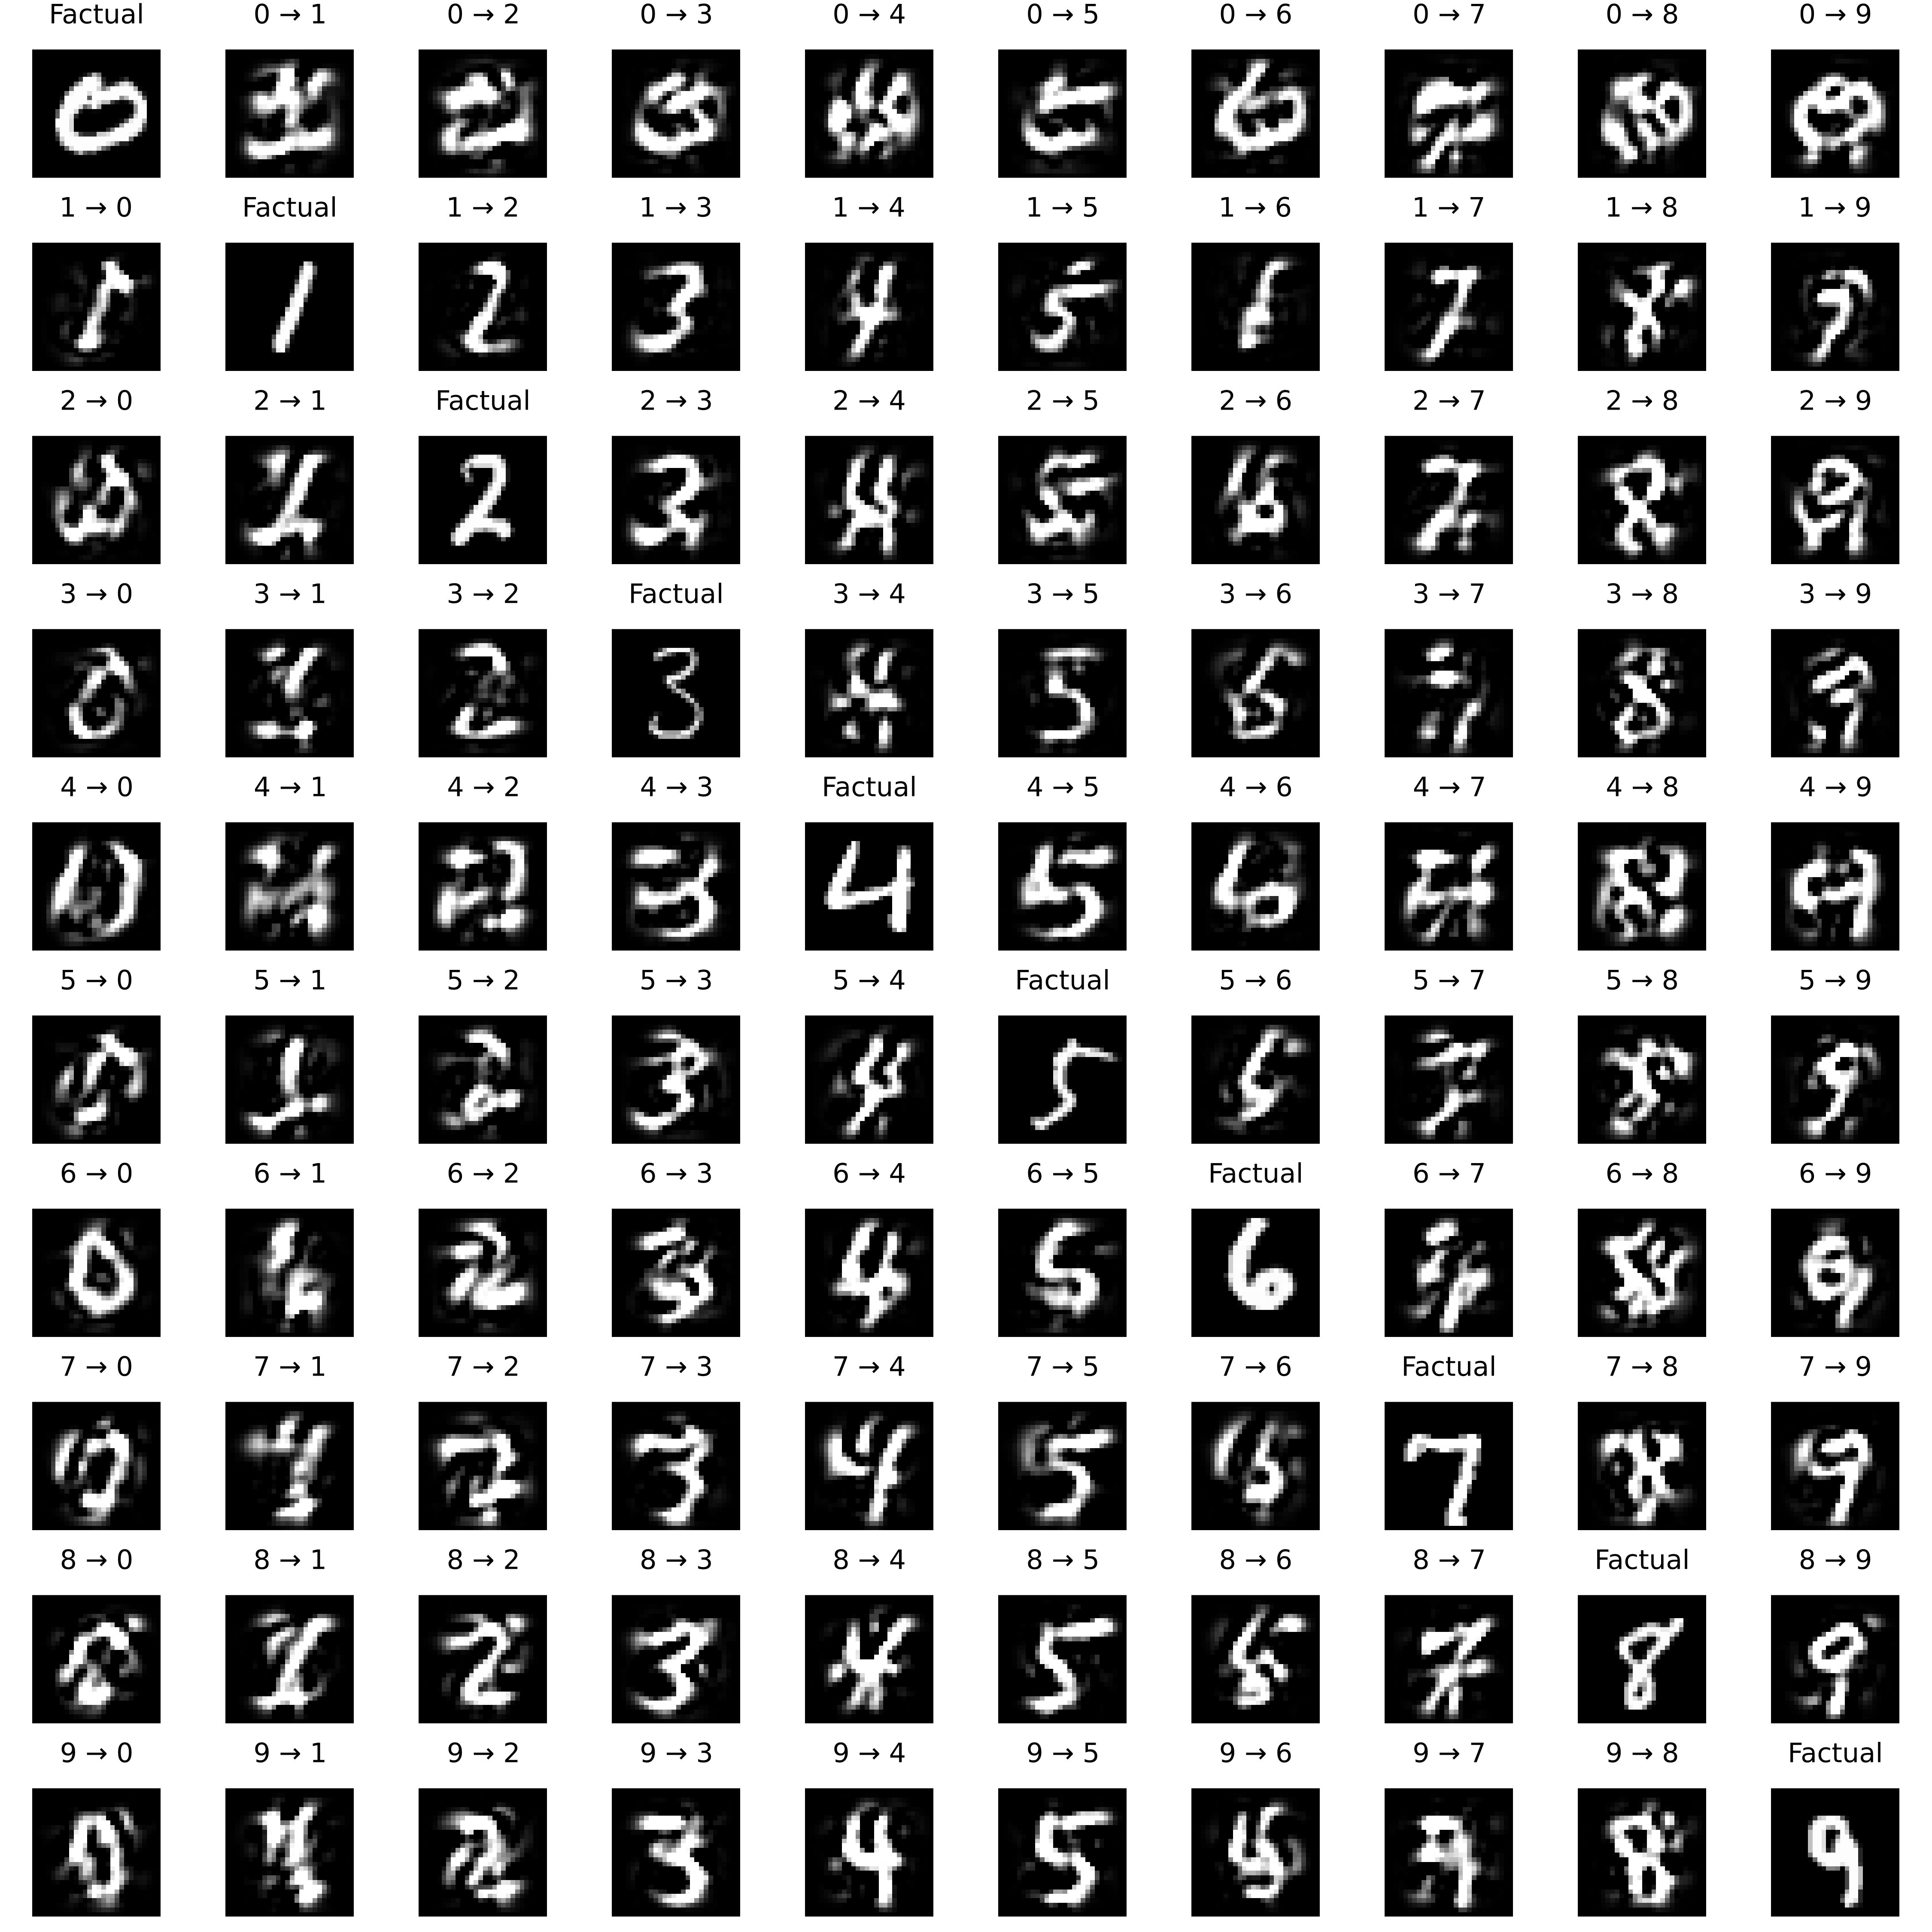
\includegraphics[width=1\textwidth,height=\textheight]{www/mnist_all_lenet_eccco.png}

}

\caption{\label{fig-mnist-lenets}Counterfactuals for LeNet-5
convolutional neural network (LeCun et al. 1998).}

\end{figure}%
\end{frame}

\begin{frame}{Example: JEM Ensemble}
\phantomsection\label{example-jem-ensemble}
\begin{figure}

\centering{


\includegraphics[width=1\textwidth,height=\textheight]{www/mnist_all_jem_ens_eccco.png}

}

\caption{\label{fig-mnist-jem}Counterfactuals for an ensemble of Joint
Energy Models (JEM) (Grathwohl et al. 2020).}

\end{figure}%
\end{frame}

\begin{frame}{Questions?}
\phantomsection\label{questions}
\begin{columns}[T]
\begin{column}{0.5\textwidth}
With thanks to my co-authors Mojtaba Farmanbar, Arie van Deursen and
Cynthia C. S. Liem.

Slides powered by \href{https://quarto.org/}{Quarto}.
\end{column}

\begin{column}{0.5\textwidth}
\end{column}
\end{columns}
\end{frame}

\begin{frame}[fragile]{Counterfactual Explanations}
\phantomsection\label{counterfactual-explanations}
All the work presented today is powered by
\href{https://github.com/JuliaTrustworthyAI/CounterfactualExplanations.jl}{\texttt{CounterfactualExplanations.jl}}
📦.

There is also a corresponding paper,
\href{https://proceedings.juliacon.org/papers/10.21105/jcon.00130}{\emph{Explaining
Black-Box Models through Counterfactuals}}, which has been published in
JuliaCon Proceedings.

If you decide to use this package in your work, please consider citing
the paper:

\href{https://doi.org/10.21105/jcon.00130}{\includesvg{presentation_files/mediabag/status.svg}}
\href{https://zenodo.org/badge/latestdoi/440782065}{\includesvg{presentation_files/mediabag/440782065.svg}}
\end{frame}

\begin{frame}[fragile]{Joint Energy Models}
\phantomsection\label{joint-energy-models}
Joint Energy Models (JEMs) are hybrid models trained to learn the
conditional output \textbf{and} input distribution (Grathwohl et al.
2020):
\href{https://github.com/JuliaTrustworthyAI/JointEnergyModels.jl}{\texttt{JointEnergyModels.jl}}
📦.

\begin{figure}

\centering{

\includegraphics{presentation_files/mediabag/www/jem.pdf}

}

\caption{\label{fig-jem}A JEM trained on Circles data.}

\end{figure}%
\end{frame}

\begin{frame}{References}
\phantomsection\label{references}
\phantomsection\label{refs}
\begin{CSLReferences}{1}{0}
\bibitem[\citeproctext]{ref-altmeyer2023explaining}
Altmeyer, Patrick, Arie van Deursen, and Cynthia Liem. 2023.
{``Explaining Black-Box Models Through Counterfactuals.''} \emph{arXiv
Preprint arXiv:2308.07198}.

\bibitem[\citeproctext]{ref-grathwohl2020your}
Grathwohl, Will, Kuan-Chieh Wang, Joern-Henrik Jacobsen, David Duvenaud,
Mohammad Norouzi, and Kevin Swersky. 2020. {``Your Classifier Is
Secretly an Energy Based Model and You Should Treat It Like One.''} In.
\url{https://openreview.net/forum?id=Hkxzx0NtDB}.

\bibitem[\citeproctext]{ref-lecun1998gradient}
LeCun, Yann, Léon Bottou, Yoshua Bengio, and Patrick Haffner. 1998.
{``Gradient-Based Learning Applied to Document Recognition.''}
\emph{Proceedings of the IEEE} 86 (11): 2278--2324.

\bibitem[\citeproctext]{ref-schut2021generating}
Schut, Lisa, Oscar Key, Rory Mc Grath, Luca Costabello, Bogdan
Sacaleanu, Yarin Gal, et al. 2021. {``Generating {Interpretable
Counterfactual Explanations By Implicit Minimisation} of {Epistemic} and
{Aleatoric Uncertainties}.''} In \emph{International {Conference} on
{Artificial Intelligence} and {Statistics}}, 1756--64. {PMLR}.

\end{CSLReferences}
\end{frame}



\end{document}
